\documentclass{beamer}
\usetheme{Singapore}
\usepackage[utf8]{inputenc}
\usecolortheme{crane}
\usepackage{graphicx}
\usepackage{iwona}
\usepackage{standalone}
\usepackage{tikz}
\usepackage{hyperref}
\usepackage{svg}

\definecolor{lightblue}{RGB}{124,190,255}
\definecolor{darkgreen}{RGB}{24,145,0}
\definecolor{darkorange}{RGB}{220,110,0}
\definecolor{colegmelyn}{RGB}{253, 198,0}

\beamertemplatenavigationsymbolsempty
\setbeamerfont{caption}{size=\tiny}

\begin{document}

\begin{frame}
  \frametitle{Geraint Palmer}
  \begin{columns}
    \begin{column}{0.5\textwidth}
      \begin{center}
        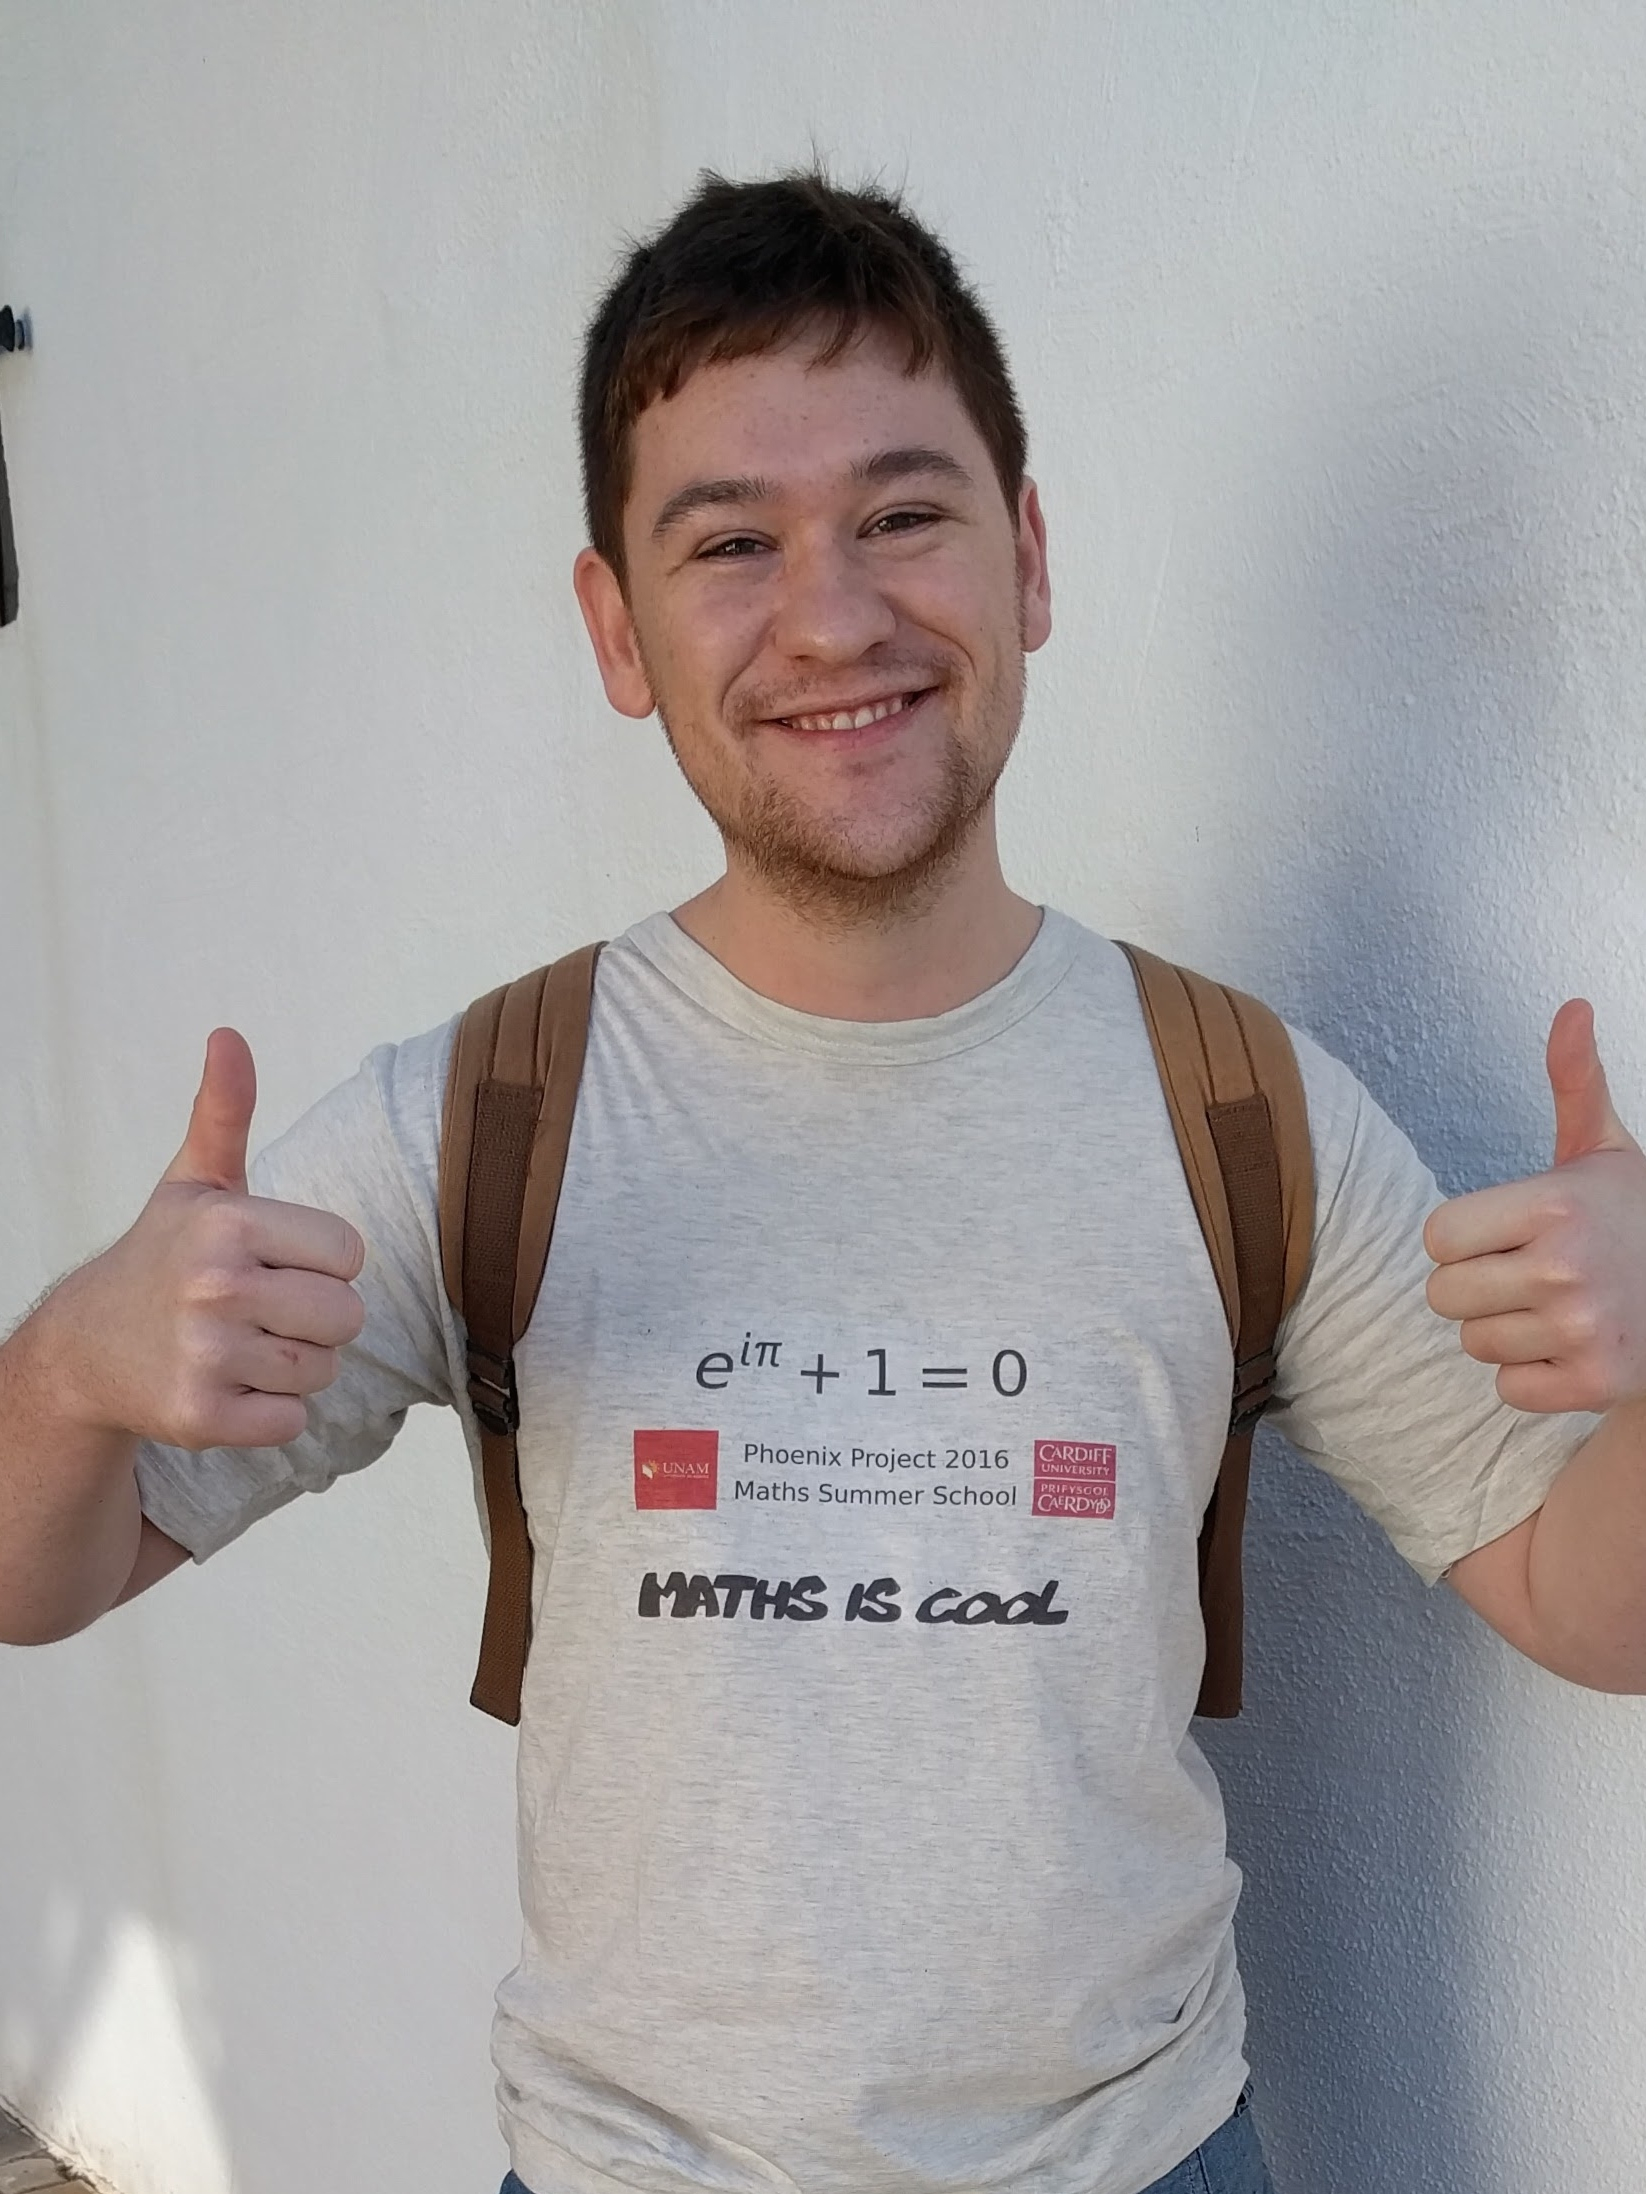
\includegraphics[width=\textwidth]{GeraintPhoto}
      \end{center}
    \end{column}
    \begin{column}{0.5\textwidth}
      \begin{center}
        Operational Research\\
        \vspace{10mm}
        Simulation, Stochastic Modelling, Queues\\
        \vspace{10mm}
        Healthcare Systems\\
      \end{center}
    \end{column}
  \end{columns}
\end{frame}

\begin{frame}
  \begin{columns}
    \begin{column}{0.5\textwidth}
      \begin{center}
        
\includegraphics[width=0.4\textwidth]{cy}\\
        \vspace{10mm}
        Software\\
        \vspace{10mm}
        Technical translation\\
      \end{center}
    \end{column}
    \begin{column}{0.5\textwidth}
      \begin{center}
        \begin{center}
          
\includegraphics[width=0.6\textwidth]{cflogo}
        \end{center}
        \vspace{7mm}
        \resizebox {0.85\columnwidth}{!}{
          \begin{tikzpicture}
            \draw[fill=colegmelyn, draw=none] (0, 0) rectangle (18, 10);
            \node at (9, 5) {
\includegraphics[width=2.5\textwidth]{CCCDu}};
          \end{tikzpicture}
        }
      \end{center}
    \end{column}
  \end{columns}
\end{frame}

\begin{frame}
\begin{center}
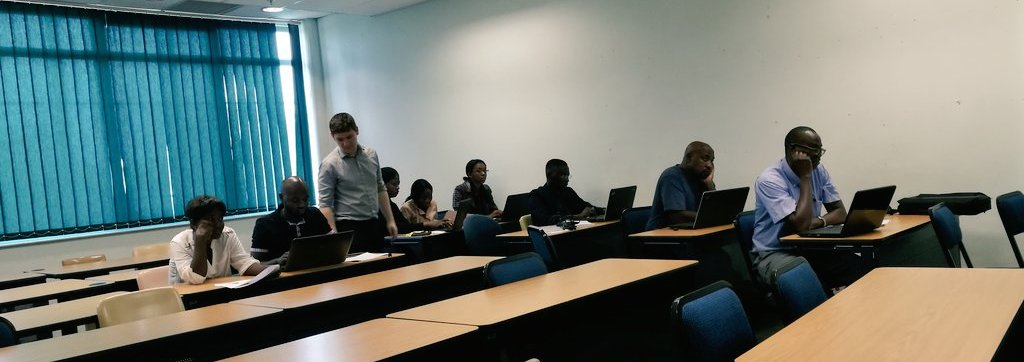
\includegraphics[width=\textwidth]{workshop}
\end{center}
\vspace{10mm}
\textcolor{darkorange}{\url{www.geraintianpalmer.org.uk} $\quad \quad$ \href{https://twitter.com/GeraintPalmer}{@GeraintPalmer}}
\end{frame}

\begin{frame}
  \frametitle{Reproducibility issues in stochastic simulation}
  \begin{center}
    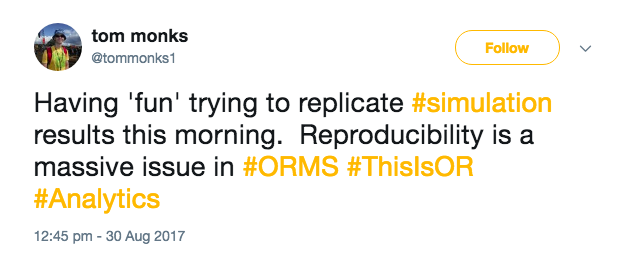
\includegraphics[width=0.8\textwidth]{reproducibility_tweet}
  \end{center}
\end{frame}

\begin{frame}
  \begin{columns}
    \begin{column}{0.6\textwidth}
      \begin{center}
          
\includegraphics[width=\textwidth]{theorsociety}
          \textit{Annual conference of the OR Society.}
          \textit{Biannual simulation workshop.}
        \end{center}
    \end{column}
    \begin{column}{0.4\textwidth}
      \begin{center}
        \resizebox {\columnwidth} {!} {
          \begin{tikzpicture}
            \draw[fill=colegmelyn, draw=none] (0, 0) rectangle (18, 10);
            \node at (9, 5) {
\includegraphics[width=3\textwidth]{CCCDu}};
          \end{tikzpicture}
        }
        \textit{Multi-disciplinary conferences.}
      \end{center}
    \end{column}
  \end{columns}
  \vspace{7mm}
  \begin{center}
    
\includegraphics[width=0.2\textwidth]{cy} 
\includegraphics[width=0.2\textwidth]{gb}\footnotemark
  \end{center}
  \footnotetext[1]{\tiny{Thanks to Twemoji.}}
\end{frame}

\end{document}
